\documentclass{article}
\usepackage{graphicx,wrapfig,hyperref,pdfpages,geometry,amsmath,longtable,eurosym,listings,textcomp}

%substitute "{\em PowerEnJoy}" with "\pej"
\newcommand{\pej}{\mbox{\normalfont\itshape PowerEnJoy }}
%substitute "{\em CSGestion}" with "\csg"
\newcommand{\csg}{\mbox{\normalfont\itshape CSGestion }}
\newcommand{\version}{\mbox{\normalfont v. 1.0 }}

%to keep the links of the TOC invisible
\hypersetup{
	colorlinks,
	citecolor=black,
	filecolor=black,
	linkcolor=black,
	urlcolor=black
}

\geometry{margin=1in}



\begin{document}

	%---------------------------	FRONT PAGE      	-----------------------------
	\title{Politecnico di Milano\\A.A. 2016/2017\\Software Engineering 2: ``{\em PowerEnJoy}'' \version \\ \bigskip \textbf{I}ntegration \textbf{T}est \textbf{P}lan \textbf{D}ocument }
	\author{Matteo Bresich (mat. 774366)}
	
	
	%to avoid the hyphenation of the name
	\hyphenation{PowerEnJoy}
	
	\begin{figure}[t]
		\centering
		\includegraphics[width=\linewidth]{"img/logo-polimi"}
		\label{fig:polimi-logo}
	\end{figure}

	\maketitle
	
	%BLANK-PAGE
	\thispagestyle{empty}
	\clearpage\mbox{}\thispagestyle{empty}\clearpage
	
	\renewcommand*\thesection{\arabic{section}}
	\renewcommand*\thesubsection{\arabic{section}.\arabic{subsection}}
	\renewcommand*\thesubsubsection{%
		\arabic{section}.\arabic{subsection}.\arabic{subsubsection}%
	}
	\setcounter{secnumdepth}{4}
	\setcounter{tocdepth}{4}
	
	%---------------------------	TABLE OF CONTENT	-----------------------------
	%to change the page numbering from roman in the toc to arabic
	\pagenumbering{roman}
	\renewcommand{\contentsname}{Table of Content}
	\tableofcontents
	
	\newpage
	\pagenumbering{arabic}
	%to insert the writing "Page" above page numbers in the TOC
	\addtocontents{toc}{~\hfill\textrm{Page}\par}
	
	%---------------------------	INTRODUCTION		-----------------------------
	\section{Introduction}
		\subsection{Revision History}
			\begin{center}
				\renewcommand{\arraystretch}{1.4}
				\begin{tabular}{ | l | l |}
					\hline
					Revision & Changes\\ \hline
					1.0 & First version of the document.\\ \hline
				\end{tabular}
			\end{center}
		\subsection{Purpose and Scope}
			The Integrated Test Planning Document describes the plan to accomplish the integration test.
			This document should be used as a reference of the testing methodologies used by the developer team. The purpose of integration testing is to verify functional, performance, and reliability requirements of individual software modules of the product when they are combined and tested as a group.
		\subsection{List of Definitions and Abbreviations}
			\subsubsection{Definitions}
			\begin{itemize}
				\item IT\textit{n}: it is the identifier of the integration test.
			\end{itemize}
			\subsubsection{Acronyms}
			\begin{itemize}
				\item RASD: Requirements Analysis and Specification Document.
				\item DD: Design Document.
				\item MOM: Message Oriented Middleware.
			\end{itemize}
		\subsection{List of Reference Documents}
			\begin{center}
				\renewcommand{\arraystretch}{1.4}
				\begin{tabular}{ | l | l | l |}
					\hline
					Revision & Document Name & File Name\\ \hline
					- & \pej Project Description & Assignments AA 2016-2017.pdf \\ \hline
					1.1 & RASD & RASD.pdf \\ \hline
					1.0 & DD & DD.pdf \\ \hline
				\end{tabular}
			\end{center}
			\pagebreak
	\section{Integration Strategy}
		\subsection{Entry Criteria}
		This section describes the prerequisites that need to be met before integration
		testing can be started. It is supposed to proceed after a successfully testing phase with a minimum coverage of 70\% of the lines of code.
		In particular the following components are considered already tested and thus trusted as working:
		\begin{itemize}
			\item Notification
			\item MOM
			\item Google Maps APIs
			\item GPS APIs
		\end{itemize}
		\subsection{Elements to be Integrated}
		Follows a scheme that shows the main high level components of the system.
		
		\begin{minipage}{\linewidth}
			\vspace{10mm}
			\makebox[\linewidth]{
				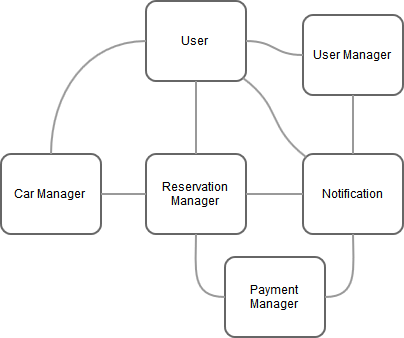
\includegraphics[keepaspectratio=true,scale=0.6]{img/elements-to-integrate}}
		\end{minipage}
		
		\pagebreak
			\begin{center}
				\renewcommand{\arraystretch}{1.4}
				\begin{tabular}{ l | p{7cm} | p{4cm} }\hline
					\multicolumn{1}{c|}{\textbf{Test ID}} & \multicolumn{1}{|c|}{\textbf{Integration Test}} & \multicolumn{1}{|c}{\textbf{Paragraphs}}\\\hline
					IT1 & Login \textrightarrow User Factory & \ref{sec:2.4.1} \hspace{20pt} \ref{sec:3.1.1} \hspace{20pt} \ref{sec:3.2.1}\\\hline
					IT2 & Profile Manager \textrightarrow Login & \ref{sec:2.4.1} \hspace{20pt} \ref{sec:3.1.1} \hspace{20pt} \ref{sec:3.2.1}\\\hline
					IT3 & Reservation Handler \textrightarrow Reservation Factory & \ref{sec:2.4.2} \hspace{20pt} \ref{sec:3.1.2} \hspace{20pt} \ref{sec:3.2.2}\\\hline
					IT4 & Reservation Handler \textrightarrow Reservation & \ref{sec:2.4.2} \hspace{20pt} \ref{sec:3.1.2} \hspace{20pt} \ref{sec:3.2.2}\\\hline
					IT5 & User \textrightarrow User Manager & \ref{sec:2.4.3} \hspace{20pt} \ref{sec:3.1.3} \hspace{20pt}\\\hline
					IT6 & User \textrightarrow Car Manager & \ref{sec:2.4.3} \hspace{20pt} \ref{sec:3.1.4} \hspace{20pt}\\\hline
					IT7 & User \textrightarrow Reservation Manager & \ref{sec:2.4.3} \hspace{20pt} \ref{sec:3.1.5} \hspace{20pt}\\\hline
					IT8 & User \textrightarrow Notification & \ref{sec:2.4.3} \hspace{20pt} \ref{sec:3.1.6} \hspace{20pt}\\\hline
					IT9 & User Manager \textrightarrow Notification & \ref{sec:2.4.4} \hspace{20pt} \ref{sec:3.1.7} \hspace{20pt}\\\hline
					IT10 & Payment Manager \textrightarrow Notification & \ref{sec:2.4.5} \hspace{20pt} \ref{sec:3.1.8} \hspace{20pt}\\\hline
					IT11 & Reservation Manager \textrightarrow Payment Manager & \ref{sec:2.4.6} \hspace{20pt} \ref{sec:3.1.9} \hspace{20pt}\\\hline
					IT12 & Reservation Manager \textrightarrow Car Manager & \ref{sec:2.4.6} \hspace{20pt} \ref{sec:3.1.10} \hspace{20pt}\\\hline
					IT13 & Reservation Manager \textrightarrow Notification & \ref{sec:2.4.6} \hspace{20pt} \ref{sec:3.1.11} \hspace{20pt}\\\hline
				\end{tabular}
			\end{center}
		\subsection{Integration Testing Strategy}
		To accomplish the analysis will be used an hybrid approach. It consists in an integration of sub-systems of the high level components followed by the integration between the high level components themselves. The choice is motivated by the fact that the development and testing in this way follows the functionality to be realized. The order of the elements to be developed is dictated by the importance of the functionality they offer.
		
		\subsection{Sequence of Component/Function Integration}
			\subsubsection{Sequence of integration for User Manager sub-system} \label{sec:2.4.1}
				\begin{minipage}{\linewidth}
					\vspace{5mm}
					\makebox[\linewidth]{
						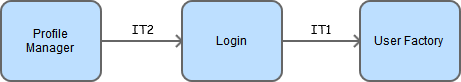
\includegraphics[keepaspectratio=true,scale=0.5]{img/integration-sequence/user-manager-subsys-integration}}
					\vspace{5mm}
				\end{minipage}
			\subsubsection{Sequence of integration for Reservation Manager sub-system} \label{sec:2.4.2}
				\begin{minipage}{\linewidth}
					\vspace{5mm}
					\makebox[\linewidth]{
						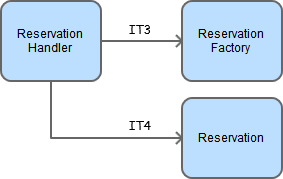
\includegraphics[keepaspectratio=true,scale=0.5]{img/integration-sequence/reservation-manager-subsys-integration}}
					\vspace{5mm}
				\end{minipage}
			\subsubsection{Sequence of integration for User} \label{sec:2.4.3}
				\begin{minipage}{\linewidth}
					\vspace{5mm}
					\makebox[\linewidth]{
						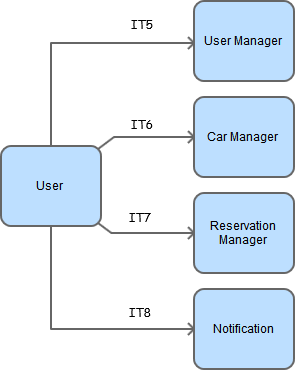
\includegraphics[keepaspectratio=true,scale=0.5]{img/integration-sequence/user-integration}}
					\vspace{5mm}
				\end{minipage}
			\subsubsection{Sequence of integration for User Manager} \label{sec:2.4.4}
			\begin{minipage}{\linewidth}
				\vspace{5mm}
				\makebox[\linewidth]{
					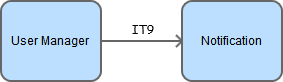
\includegraphics[keepaspectratio=true,scale=0.5]{img/integration-sequence/user-manager-notification-integration}}
				\vspace{5mm}
			\end{minipage}
			\subsubsection{Sequence of integration for Payment Manager} \label{sec:2.4.5}
			\begin{minipage}{\linewidth}
				\vspace{5mm}
				\makebox[\linewidth]{
					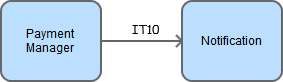
\includegraphics[keepaspectratio=true,scale=0.5]{img/integration-sequence/payment-manager-notification-integration}}
				\vspace{5mm}
			\end{minipage}
			\subsubsection{Sequence of integration for Reservation Manager} \label{sec:2.4.6}
			\begin{minipage}{\linewidth}
				\vspace{5mm}
				\makebox[\linewidth]{
					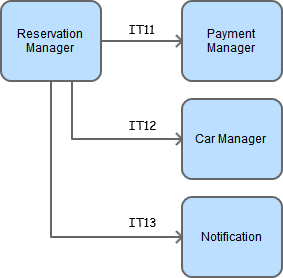
\includegraphics[keepaspectratio=true,scale=0.5]{img/integration-sequence/reservation-manager-integration}}
			\end{minipage}
	\section{Individual Steps and Test Description}
		\subsection{Integration Test Case Specifications}
			\subsubsection{Integration Test for User Manager sub-system} \label{sec:3.1.1}
				\begin{minipage}{\linewidth}
					\makebox[\linewidth]{
						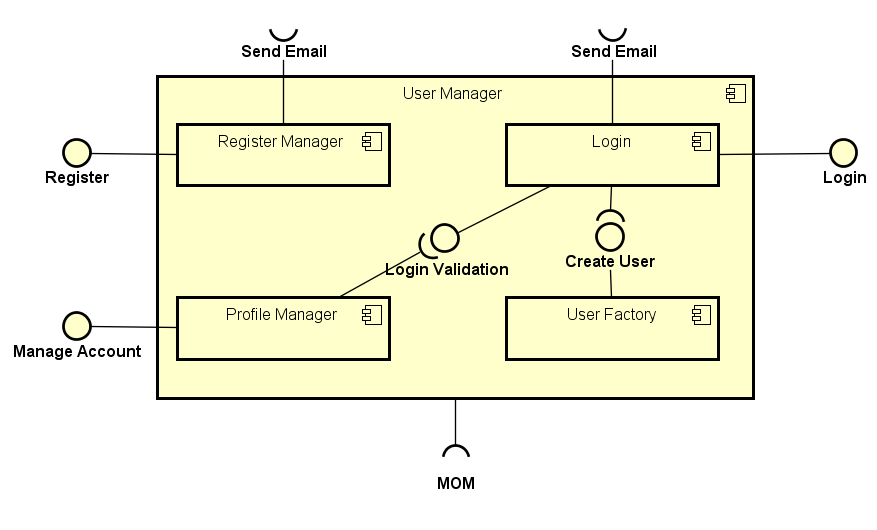
\includegraphics[keepaspectratio=true,scale=0.5]{../DD/img/components-detail/user-manager}}
				\end{minipage}
				\begin{center}
					Image taken from the Design Document (paragraph 2.3.1)
				\end{center}
				\begin{center}
					\setlength{\tabcolsep}{24pt}
					\renewcommand{\arraystretch}{1.4}
					\begin{tabular}{ | l | p{8cm} |}\hline
						\textbf{Test case identifier} & IT1\\\hline
						\textbf{Test items} & Login \textrightarrow User Factory\\\hline
						\textbf{Input specification} & Methods call from Login to User Factory with typical input \\\hline
						\textbf{Output specification} & Check the correctness of User Factory's methods  \\\hline
						\textbf{Environmental needs} & User Driver, MOM and Notification Stub\\\hline
					\end{tabular}
				\end{center}	
				\bigskip
				\begin{center}
					\setlength{\tabcolsep}{24pt}
					\renewcommand{\arraystretch}{1.4}
					\begin{tabular}{ | l | p{8cm} |}\hline
						\textbf{Test case identifier} & IT2\\\hline
						\textbf{Test items} & Profile Manager \textrightarrow Login\\\hline
						\textbf{Input specification} & Methods call from Profile Manager to Login with typical input \\\hline
						\textbf{Output specification} & Check the correctness of Login's methods \\\hline
						\textbf{Environmental needs} & User Driver, MOM and Notification Stub\\\hline
					\end{tabular}
				\end{center}
			\subsubsection{Integration Test for Reservation Manager sub-system} \label{sec:3.1.2}
				\begin{minipage}{\linewidth}
					\makebox[\linewidth]{
						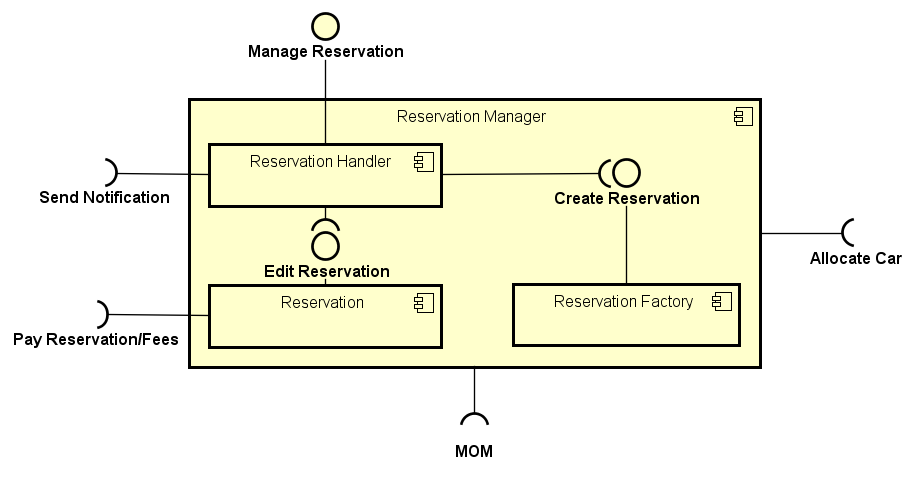
\includegraphics[keepaspectratio=true,scale=0.5]{../DD/img/components-detail/reservation-manager}}
				\end{minipage}
				\begin{center}
					Image taken from the Design Document (paragraph 2.3.3)
				\end{center}
				\begin{center}
					\setlength{\tabcolsep}{24pt}
					\renewcommand{\arraystretch}{1.4}
					\begin{tabular}{ | l | p{8cm} |}\hline
						\textbf{Test case identifier} & IT3\\\hline
						\textbf{Test items} & Reservation Handler \textrightarrow Reservation Factory\\\hline
						\textbf{Input specification} &  Methods call from Reservation Handler to Reservation Factory with typical input \\\hline
						\textbf{Output specification} & Check the correctness of Reservation Factory's methods \\\hline
						\textbf{Environmental needs} & User Driver, MOM and Car Manager Stub \\\hline
					\end{tabular}
				\end{center}	
				\bigskip
				\begin{center}
					\setlength{\tabcolsep}{24pt}
					\renewcommand{\arraystretch}{1.4}
					\begin{tabular}{ | l | p{8cm} |}\hline
						\textbf{Test case identifier} & IT4\\\hline
						\textbf{Test items} & Reservation Handler \textrightarrow Reservation\\\hline
						\textbf{Input specification} & Methods call from Reservation Handler to Reservation with typical input \\\hline
						\textbf{Output specification} & Check the correctness of Reservation's methods \\\hline
						\textbf{Environmental needs} & User Driver, MOM and Car Manager Stub \\\hline
					\end{tabular}
				\end{center}
				\pagebreak
			\subsubsection{Integration Test for User and User Manager} \label{sec:3.1.3}
				\begin{minipage}{\linewidth}
					\makebox[\linewidth]{
						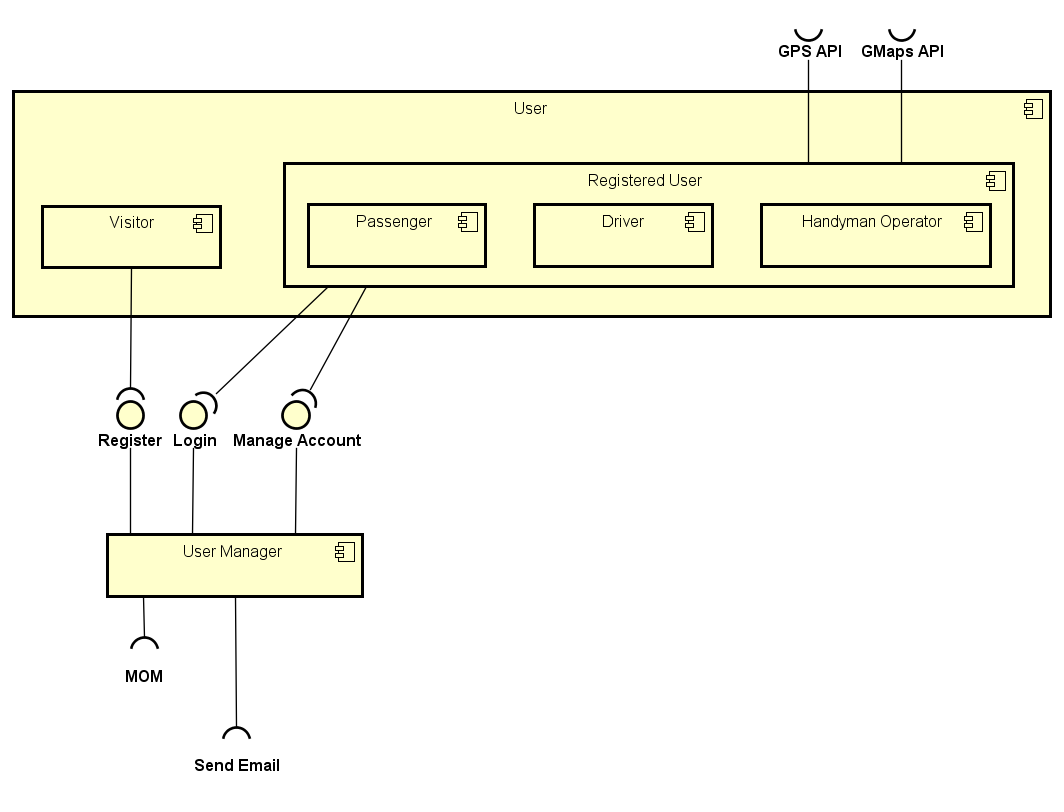
\includegraphics[keepaspectratio=true,scale=0.4]{img/integration-test/user-user-manager}}
				\end{minipage}
				\begin{center}
					\setlength{\tabcolsep}{24pt}
					\renewcommand{\arraystretch}{1.4}
					\begin{tabular}{ | l | p{8cm} |}\hline
						\textbf{Test case identifier} & IT5\\\hline
						\textbf{Test items} & User \textrightarrow User Manager\\\hline
						\textbf{Input specification} & Methods call from User to User Manager with typical input \\\hline
						\textbf{Output specification} & Check the correctness of User Manager's methods \\\hline
						\textbf{Environmental needs} & IT1 and IT2 passed, User Driver and MOM \\\hline
					\end{tabular}
				\end{center}
				\pagebreak
			\subsubsection{Integration Test for User and Car Manager} \label{sec:3.1.4}
				\begin{minipage}{\linewidth}
				\makebox[\linewidth]{
					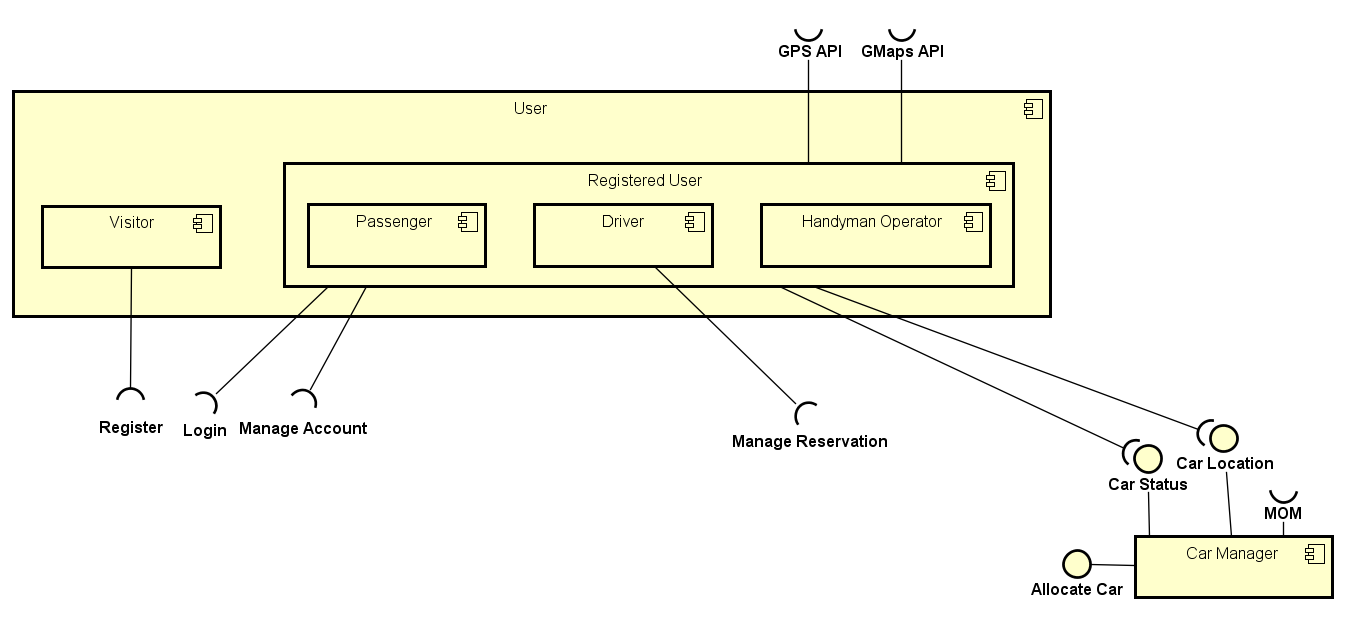
\includegraphics[keepaspectratio=true,scale=0.4]{img/integration-test/user-car-manager}}
				\end{minipage}
				\begin{center}
					\setlength{\tabcolsep}{24pt}
					\renewcommand{\arraystretch}{1.4}
					\begin{tabular}{ | l | p{8cm} |}\hline
						\textbf{Test case identifier} & IT6\\\hline
						\textbf{Test items} & User \textrightarrow Car Manager\\\hline
						\textbf{Input specification} & Methods call from User to Car Manager with typical input \\\hline
						\textbf{Output specification} & Check the correctness of Car Manager's methods \\\hline
						\textbf{Environmental needs} & User Driver and MOM\\\hline
					\end{tabular}
				\end{center}
				\pagebreak
			\subsubsection{Integration Test for User and Reservation Manager} \label{sec:3.1.5}
				\begin{minipage}{\linewidth}
				\makebox[\linewidth]{
					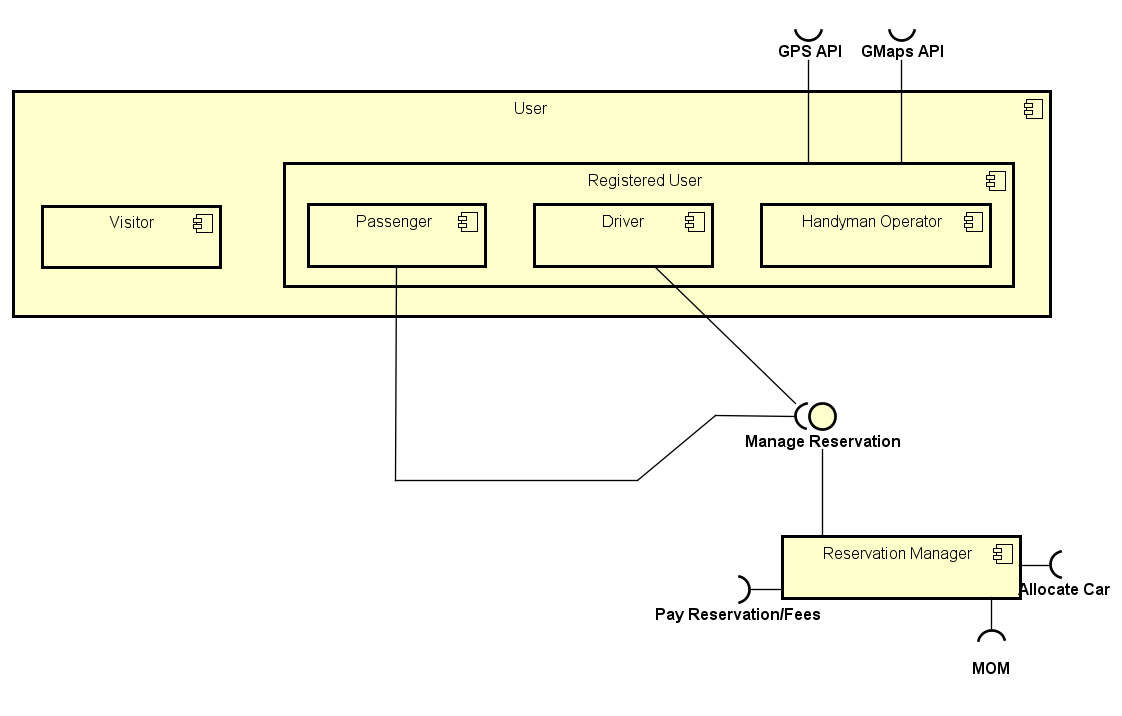
\includegraphics[keepaspectratio=true,scale=0.4]{img/integration-test/user-reservation-manager}}
				\end{minipage}
				\begin{center}
					\setlength{\tabcolsep}{24pt}
					\renewcommand{\arraystretch}{1.4}
					\begin{tabular}{ | l | p{8cm} |}\hline
						\textbf{Test case identifier} & IT7\\\hline
						\textbf{Test items} & User \textrightarrow Reservation Manager\\\hline
						\textbf{Input specification} & Methods call from User to Reservation Manager with typical input \\\hline
						\textbf{Output specification} & Check the correctness of Reservation Manager's methods \\\hline
						\textbf{Environmental needs} & IT3 and IT4 passed, User Driver, Payment Manager Stub and MOM \\\hline
					\end{tabular}
				\end{center}
				\pagebreak
			\subsubsection{Integration Test for User and Notification} \label{sec:3.1.6}
				\begin{minipage}{\linewidth}
				\makebox[\linewidth]{
					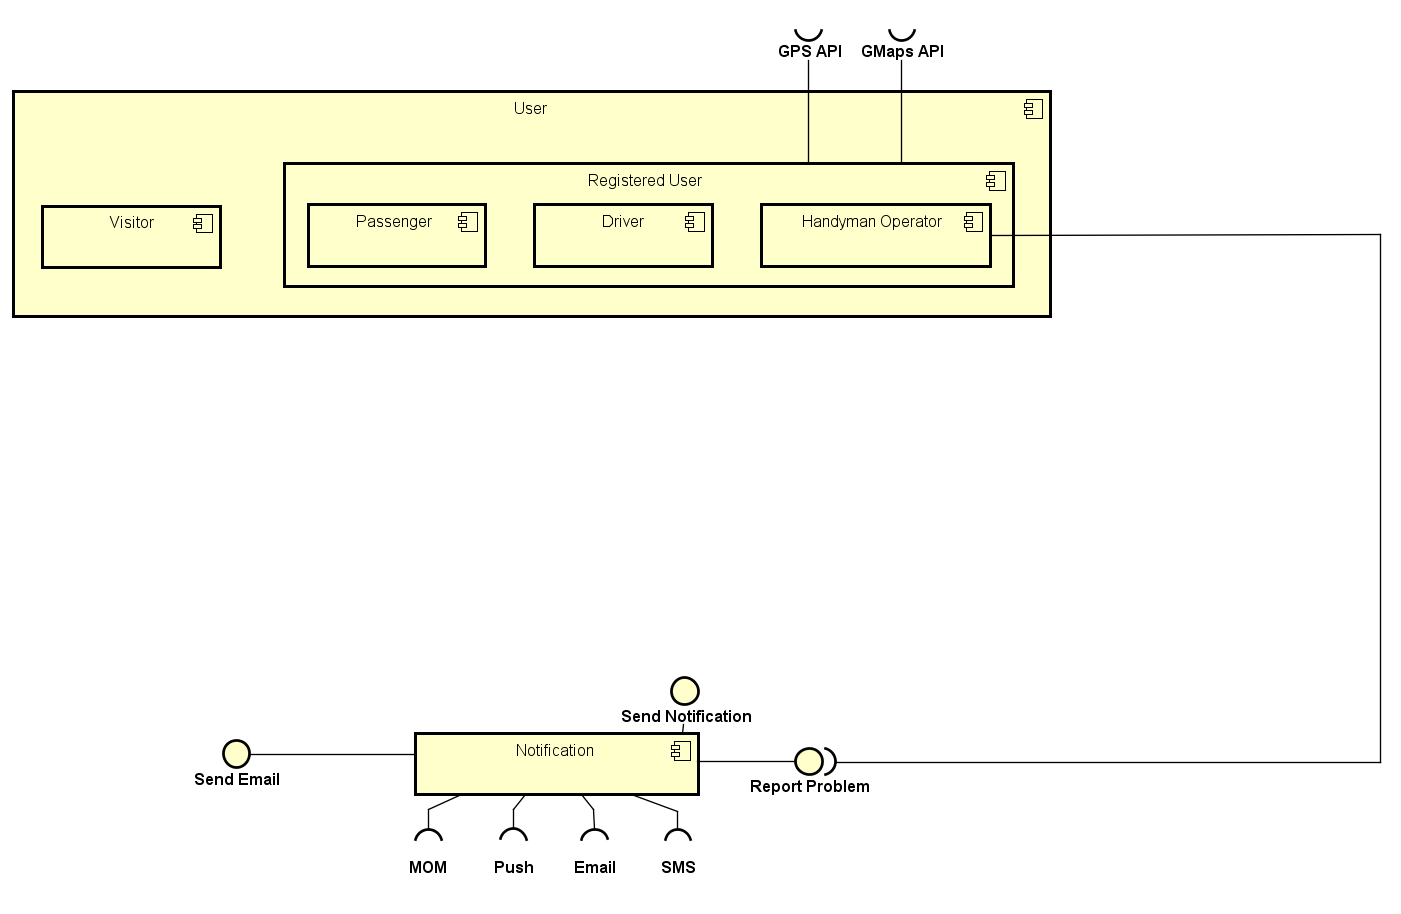
\includegraphics[keepaspectratio=true,scale=0.4]{img/integration-test/user-notification}}
				\end{minipage}
				\begin{center}
					\setlength{\tabcolsep}{24pt}
					\renewcommand{\arraystretch}{1.4}
					\begin{tabular}{ | l | p{8cm} |}\hline
						\textbf{Test case identifier} & IT8\\\hline
						\textbf{Test items} & User \textrightarrow Notification\\\hline
						\textbf{Input specification} & Methods call from User to Notification with typical input \\\hline
						\textbf{Output specification} & Check the correctness of Notification's methods\\\hline
						\textbf{Environmental needs} & User Driver and MOM, Email, SMS and Push notification stubs \\\hline
					\end{tabular}
				\end{center}
				\pagebreak
			\subsubsection{Integration Test for User Manager and Notification} \label{sec:3.1.7}
				\begin{minipage}{\linewidth}
					\makebox[\linewidth]{
						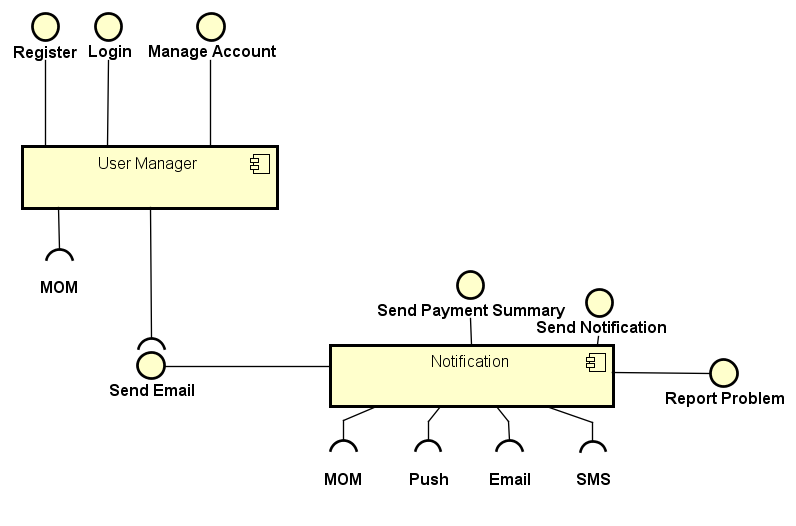
\includegraphics[keepaspectratio=true,scale=0.5]{img/integration-test/user-manager-notification}}
				\end{minipage}
				\begin{center}
					\setlength{\tabcolsep}{24pt}
					\renewcommand{\arraystretch}{1.4}
					\begin{tabular}{ | l | p{8cm} |}\hline
						\textbf{Test case identifier} & IT9\\\hline
						\textbf{Test items} & User Manager \textrightarrow Notification\\\hline
						\textbf{Input specification} & Methods call from User Manager to Notification with typical input \\\hline
						\textbf{Output specification} & Check the correctness of Notification's methods \\\hline
						\textbf{Environmental needs} & IT1 and IT2 passed, User Driver and MOM, Email, SMS and Push notification stubs \\\hline
					\end{tabular}
				\end{center}
				\pagebreak
			\subsubsection{Integration Test for Payment Manager and Notification} \label{sec:3.1.8}
				\begin{minipage}{\linewidth}
				\makebox[\linewidth]{
					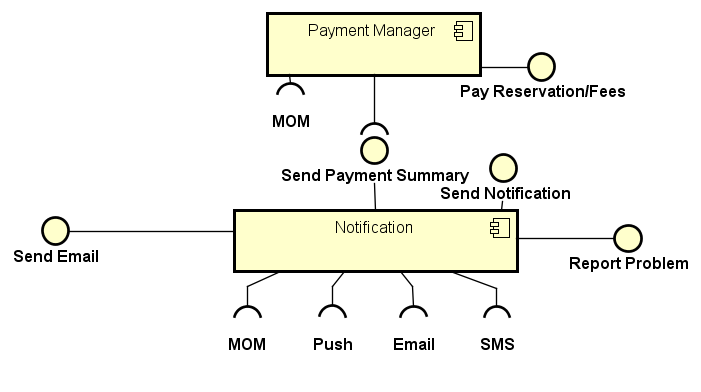
\includegraphics[keepaspectratio=true,scale=0.5]{img/integration-test/payment-manager-notification}}
				\end{minipage}
				\begin{center}
					\setlength{\tabcolsep}{24pt}
					\renewcommand{\arraystretch}{1.4}
					\begin{tabular}{ | l | p{8cm} |}\hline
						\textbf{Test case identifier} & IT10\\\hline
						\textbf{Test items} & Payment Manager \textrightarrow Notification\\\hline
						\textbf{Input specification} & Methods call from Payment Manager to Notification with typical input \\\hline
						\textbf{Output specification} & Check the correctness of Notification's methods \\\hline
						\textbf{Environmental needs} & Reservation Manager Driver, MOM, Email, SMS and Push notification stubs \\\hline
					\end{tabular}
				\end{center}
				\pagebreak
			\subsubsection{Integration Test for Reservation Manager and Payment Manager} \label{sec:3.1.9}
				\begin{minipage}{\linewidth}
				\makebox[\linewidth]{
					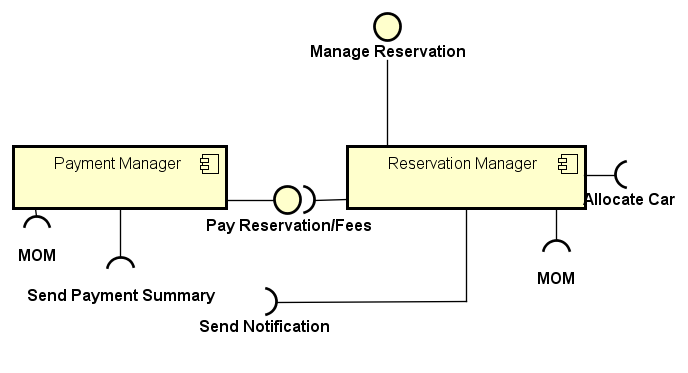
\includegraphics[keepaspectratio=true,scale=0.5]{img/integration-test/reservation-manager-payment-manager}}
				\end{minipage}
				\begin{center}
					\setlength{\tabcolsep}{24pt}
					\renewcommand{\arraystretch}{1.4}
					\begin{tabular}{ | l | p{8cm} |}\hline
						\textbf{Test case identifier} & IT11\\\hline
						\textbf{Test items} & Reservation Manager \textrightarrow Payment Manager\\\hline
						\textbf{Input specification} & Methods call from Reservation Manager to Payment Manager with typical input \\\hline
						\textbf{Output specification} & Check the correctness of Payment Manager's methods \\\hline
						\textbf{Environmental needs} & IT3 and IT4 passed, MOM, Car Manager and Notification Stubs \\\hline
					\end{tabular}
				\end{center}
				\pagebreak
			\subsubsection{Integration Test for Reservation Manager and Car Manager} \label{sec:3.1.10}
				\begin{minipage}{\linewidth}
				\makebox[\linewidth]{
					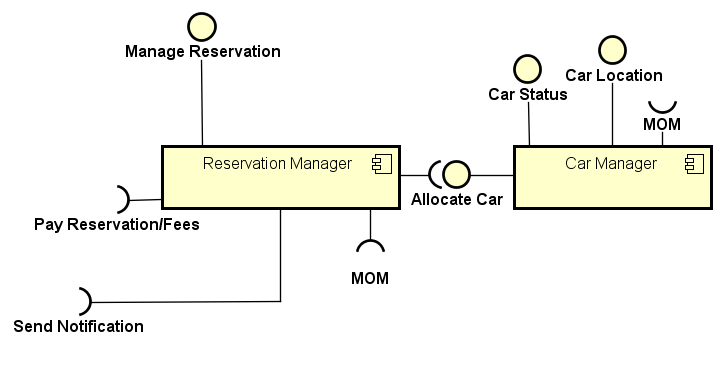
\includegraphics[keepaspectratio=true,scale=0.5]{img/integration-test/reservation-manager-car-manager}}
				\end{minipage}
				\begin{center}
					\setlength{\tabcolsep}{24pt}
					\renewcommand{\arraystretch}{1.4}
					\begin{tabular}{ | l | p{8cm} |}\hline
						\textbf{Test case identifier} & IT12\\\hline
						\textbf{Test items} & Reservation Manager \textrightarrow Car Manager\\\hline
						\textbf{Input specification} & Methods call from Reservation Manager to Car Manager with typical input \\\hline
						\textbf{Output specification} & Check the correctness of Car Manager's methods \\\hline
						\textbf{Environmental needs} & IT3 and IT4 passed, MOM, Payment Manager and Notification Stubs \\\hline
					\end{tabular}
				\end{center}
				\pagebreak
			\subsubsection{Integration Test for Reservation Manager and Notification} \label{sec:3.1.11}
				\begin{minipage}{\linewidth}
					\makebox[\linewidth]{
						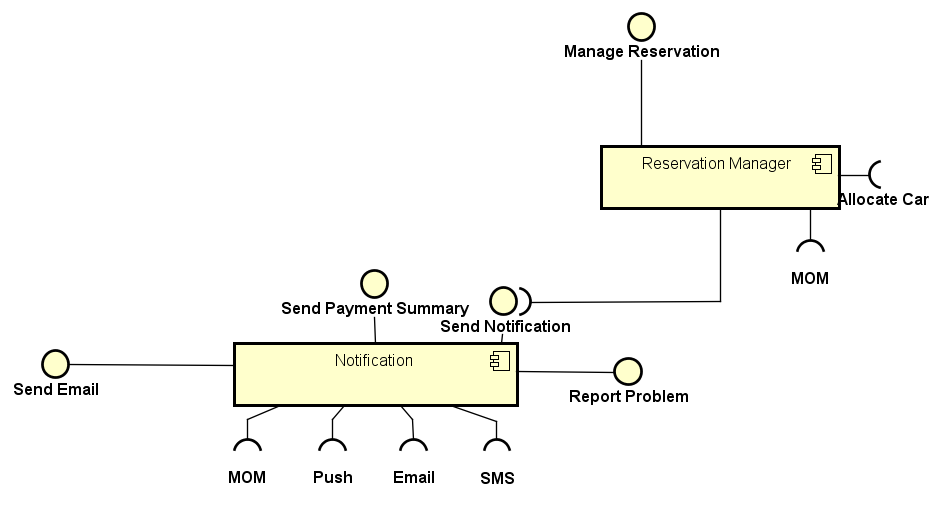
\includegraphics[keepaspectratio=true,scale=0.5]{img/integration-test/reservation-manager-notification}}
				\end{minipage}
				\begin{center}
					\setlength{\tabcolsep}{24pt}
					\renewcommand{\arraystretch}{1.4}
					\begin{tabular}{ | l | p{8cm} |}\hline
						\textbf{Test case identifier} & IT13\\\hline
						\textbf{Test items} & Reservation Manager \textrightarrow Notification\\\hline
						\textbf{Input specification} & Methods call from Reservation Manager to Notification with typical input \\\hline
						\textbf{Output specification} & Check the correctness of Notification's methods \\\hline
						\textbf{Environmental needs} & User Driver, MOM, Email, SMS and Push notification stubs \\\hline
					\end{tabular}
				\end{center}
			\pagebreak
		\subsection{Test procedures}
			\subsubsection{Test procedure for User Manager sub-system} \label{sec:3.2.1}
				\begin{center}
					\setlength{\tabcolsep}{24pt}
					\renewcommand{\arraystretch}{1.4}
					\begin{tabular}{ | l | p{8cm} |}\hline
						\textbf{Test procedure identifier} & TP1\\\hline
						\textbf{Purpose} & This test verifies that the User Manager component:
							\begin{itemize}
								\item Can handle user input
								\item Can output the requested information to a user
								\item Can modify informations about a user
								\item Can retrieve the correct information about a user
							\end{itemize} \\\hline
						\textbf{Procedure steps} & Execute in order IT1 and IT2 \\\hline
					\end{tabular}
				\end{center}
			\subsubsection{Test procedure for Reservation Manager sub-system} \label{sec:3.2.2}
				\begin{center}
					\setlength{\tabcolsep}{24pt}
					\renewcommand{\arraystretch}{1.4}
					\begin{tabular}{ | l | p{8cm} |}\hline
						\textbf{Test procedure identifier} & TP2\\\hline
						\textbf{Purpose} & This test verifies that the Reservation Manager component:
						\begin{itemize}
							\item Can handle the creation, modification and cancellation of rides
							\item Can handle the creation, modification and cancellation of seats reservations
							\item Can handle payment process
							\item Can retrieve information about the rides
							\item Can send notifications to users
						\end{itemize} \\\hline
						\textbf{Procedure steps} & Execute in order IT3 and IT4 \\\hline
					\end{tabular}
				\end{center}
				\pagebreak
			\subsubsection{Test procedure for components involved in user login} \label{sec:3.2.3}
				\begin{minipage}{\linewidth}
					\makebox[\linewidth]{
						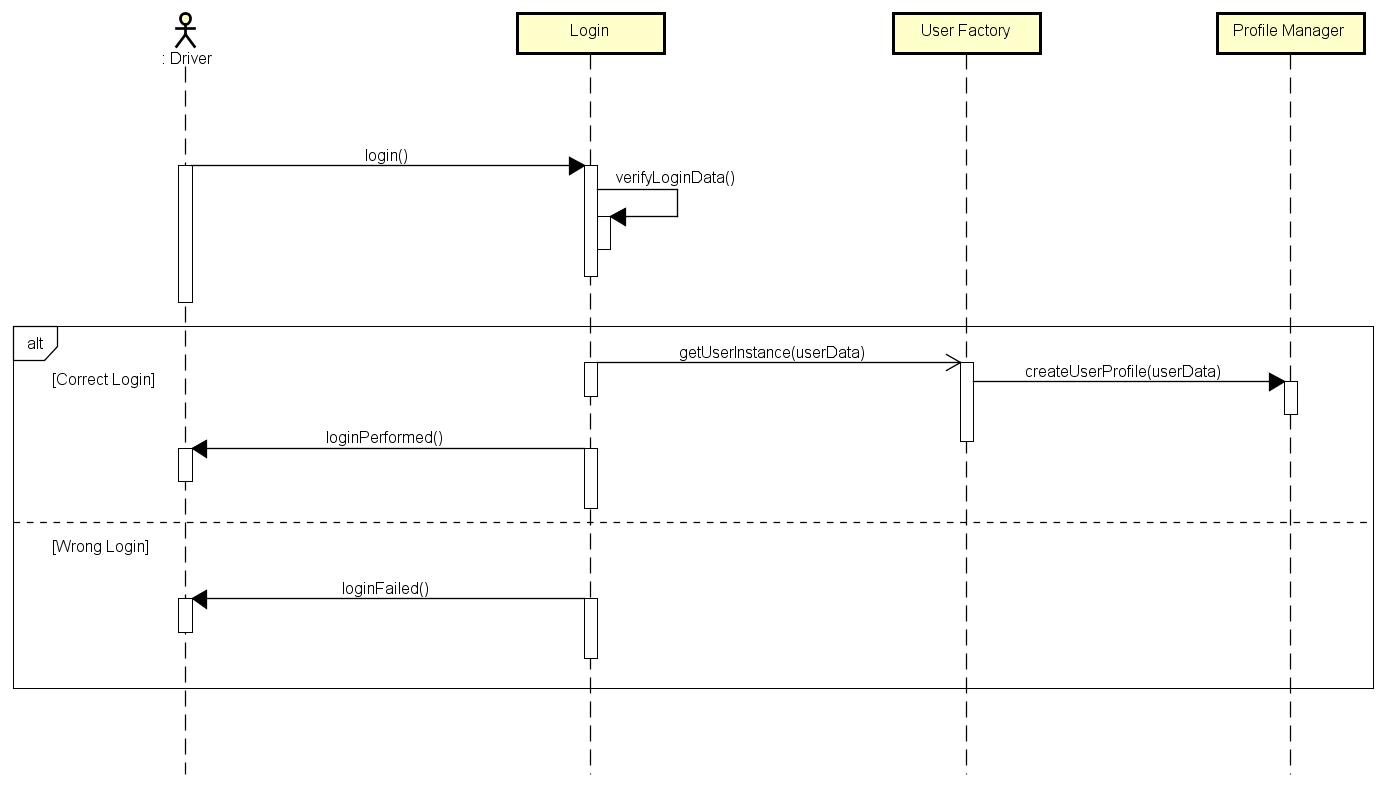
\includegraphics[keepaspectratio=true,scale=0.5]{../DD/img/sequence-diagram/login}}
				\end{minipage}
				\begin{center}
					Image taken from the Design Document (paragraph 2.5.2.1)
				\end{center}
				\begin{center}
					\setlength{\tabcolsep}{24pt}
					\renewcommand{\arraystretch}{1.4}
					\begin{tabular}{ | l | p{8cm} |}\hline
						\textbf{Test procedure identifier} & TP3\\\hline
						\textbf{Purpose} & This test verifies the login procedure. The purpose of the procedure is to check the correct integration of all the involved components: Login, User Factory and Profile Manager. \\\hline
						\textbf{Procedure steps} & IT1 followed by IT2 \\\hline
					\end{tabular}
				\end{center}
			\subsubsection{Test procedure for components involved in car/seat reservation} \label{sec:3.2.4}
				\begin{minipage}{\linewidth}
					\makebox[\linewidth]{
						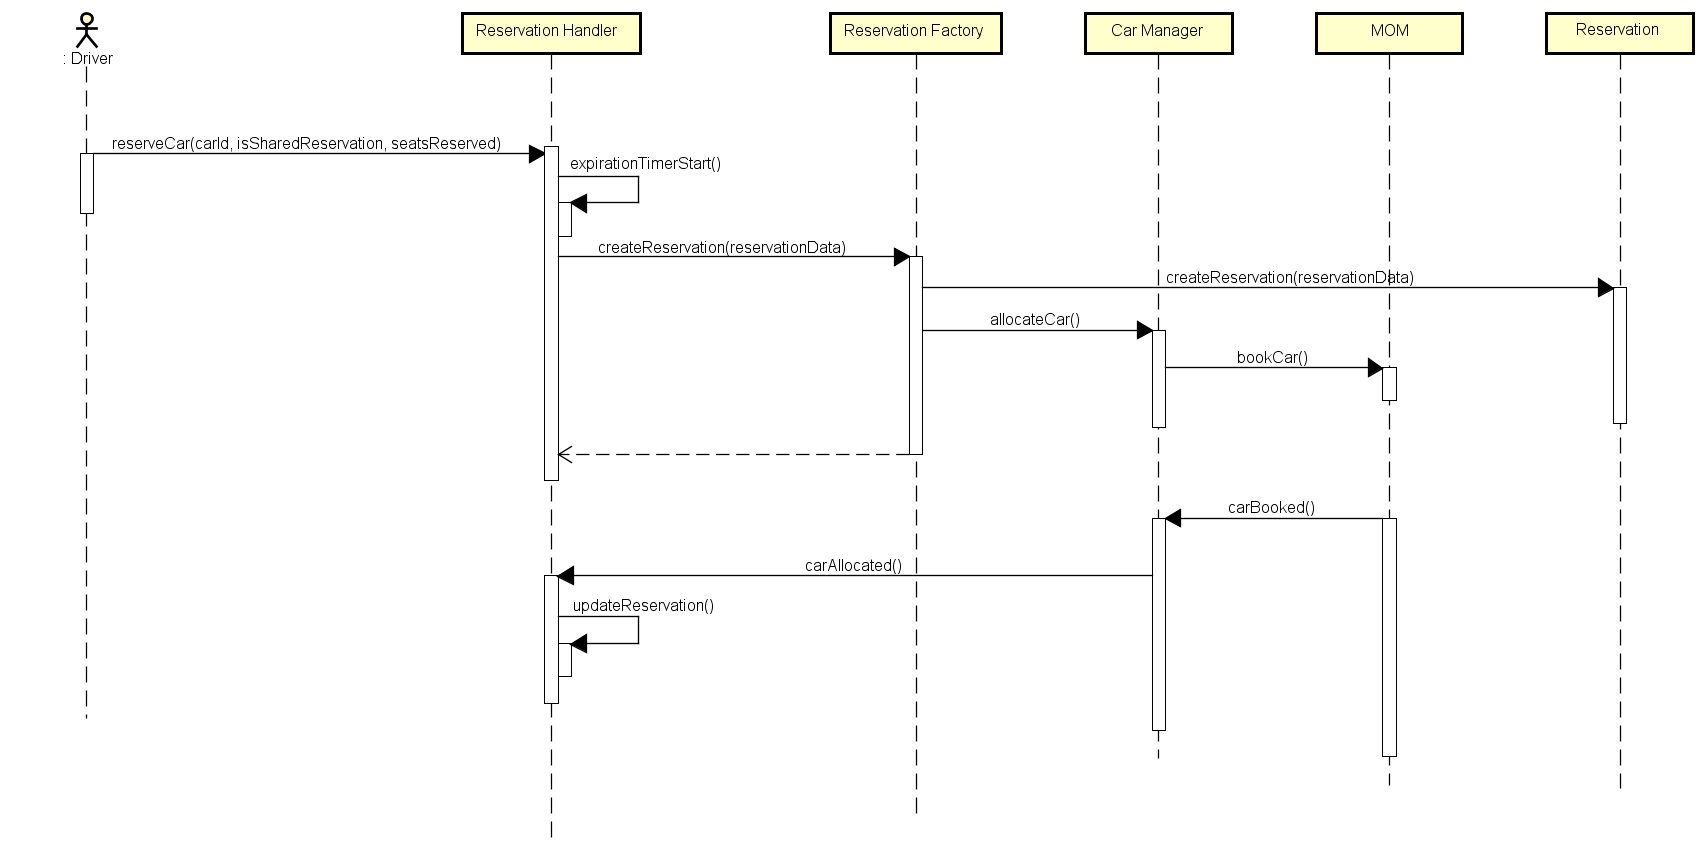
\includegraphics[keepaspectratio=true,scale=0.4]{../DD/img/sequence-diagram/car-reservation}}
				\end{minipage}
				\begin{center}
					Image taken from the Design Document (paragraph 2.5.2.2)
				\end{center}
				\begin{center}
					\setlength{\tabcolsep}{24pt}
					\renewcommand{\arraystretch}{1.4}
					\begin{tabular}{ | l | p{8cm} |}\hline
						\textbf{Test procedure identifier} & TP4\\\hline
						\textbf{Purpose} & This test verifies the car reservation procedure. The purpose of the procedure is to check the correct integration of all the involved components: Reservation Handler, Reservation Factory, Car Manager, MOM and Reservation. \\\hline
						\textbf{Procedure steps} & Execute in order IT3, IT4, IT12 \\\hline
					\end{tabular}
				\end{center}
				\pagebreak
				\begin{minipage}{\linewidth}
					\makebox[\linewidth]{
						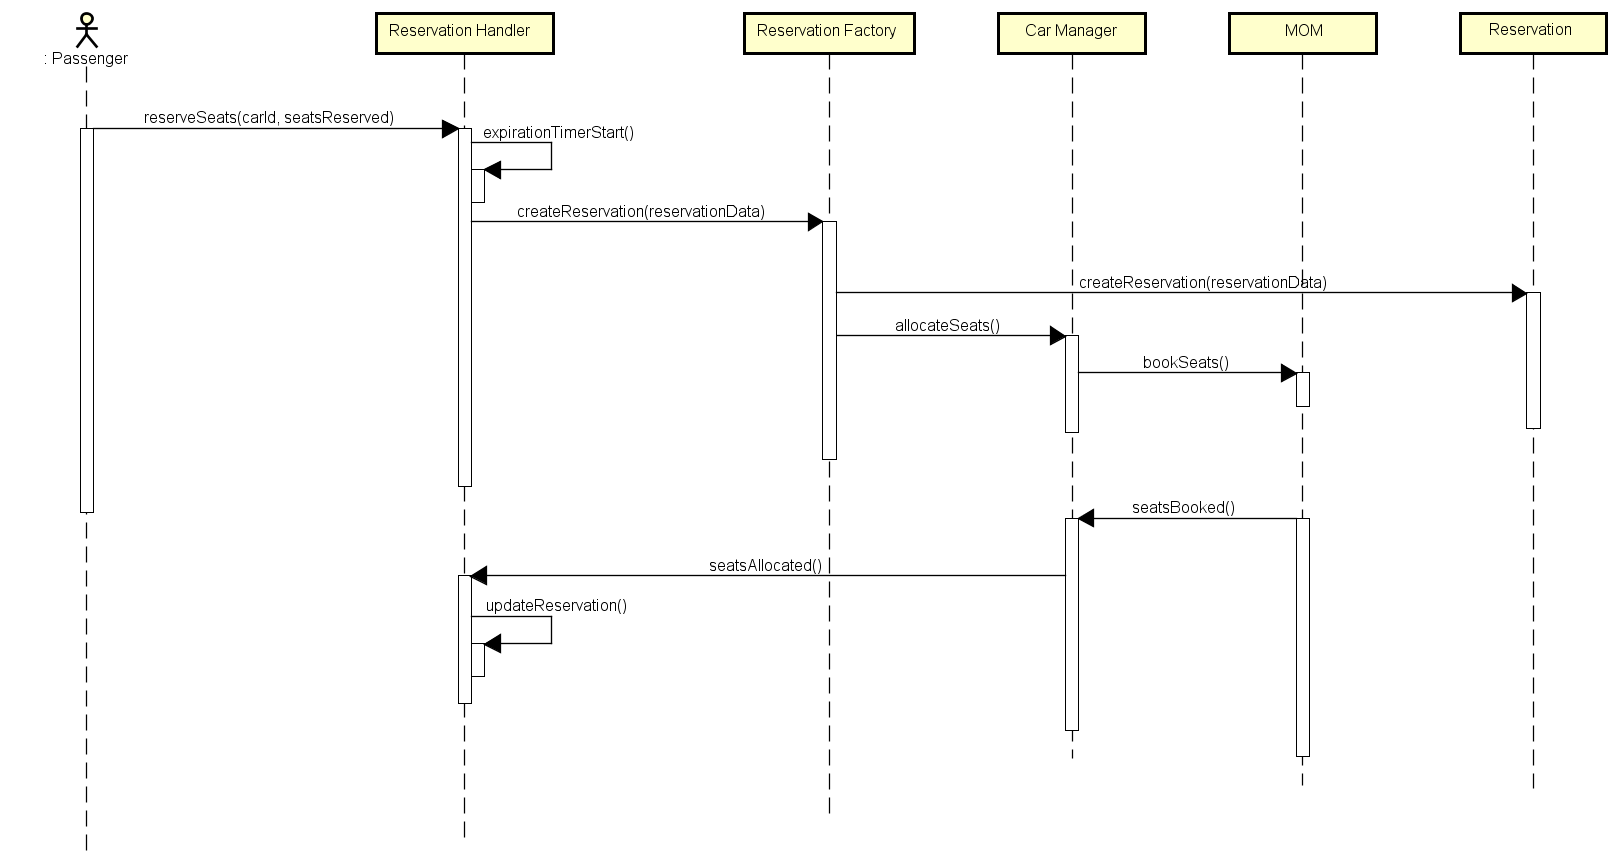
\includegraphics[keepaspectratio=true,scale=0.42]{../DD/img/sequence-diagram/seat-reservation}}
				\end{minipage}
				\begin{center}
					Image taken from the Design Document (paragraph 2.5.2.3)
				\end{center}
				\begin{center}
					\setlength{\tabcolsep}{24pt}
					\renewcommand{\arraystretch}{1.4}
					\begin{tabular}{ | l | p{8cm} |}\hline
						\textbf{Test procedure identifier} & TP5\\\hline
						\textbf{Purpose} & This test verifies the seat reservation procedure. The purpose of the procedure is to check the correct integration of all the involved components: Reservation Handler, Reservation Factory, Car Manager, MOM and Reservation. \\\hline
						\textbf{Procedure steps} & Execute in order IT3, IT4, IT12 \\\hline
					\end{tabular}
				\end{center}
				\pagebreak
			\subsubsection{Test procedure for components involved in delete a car reservation} \label{sec:3.2.5}
			\begin{minipage}{\linewidth}
				\makebox[\linewidth]{
					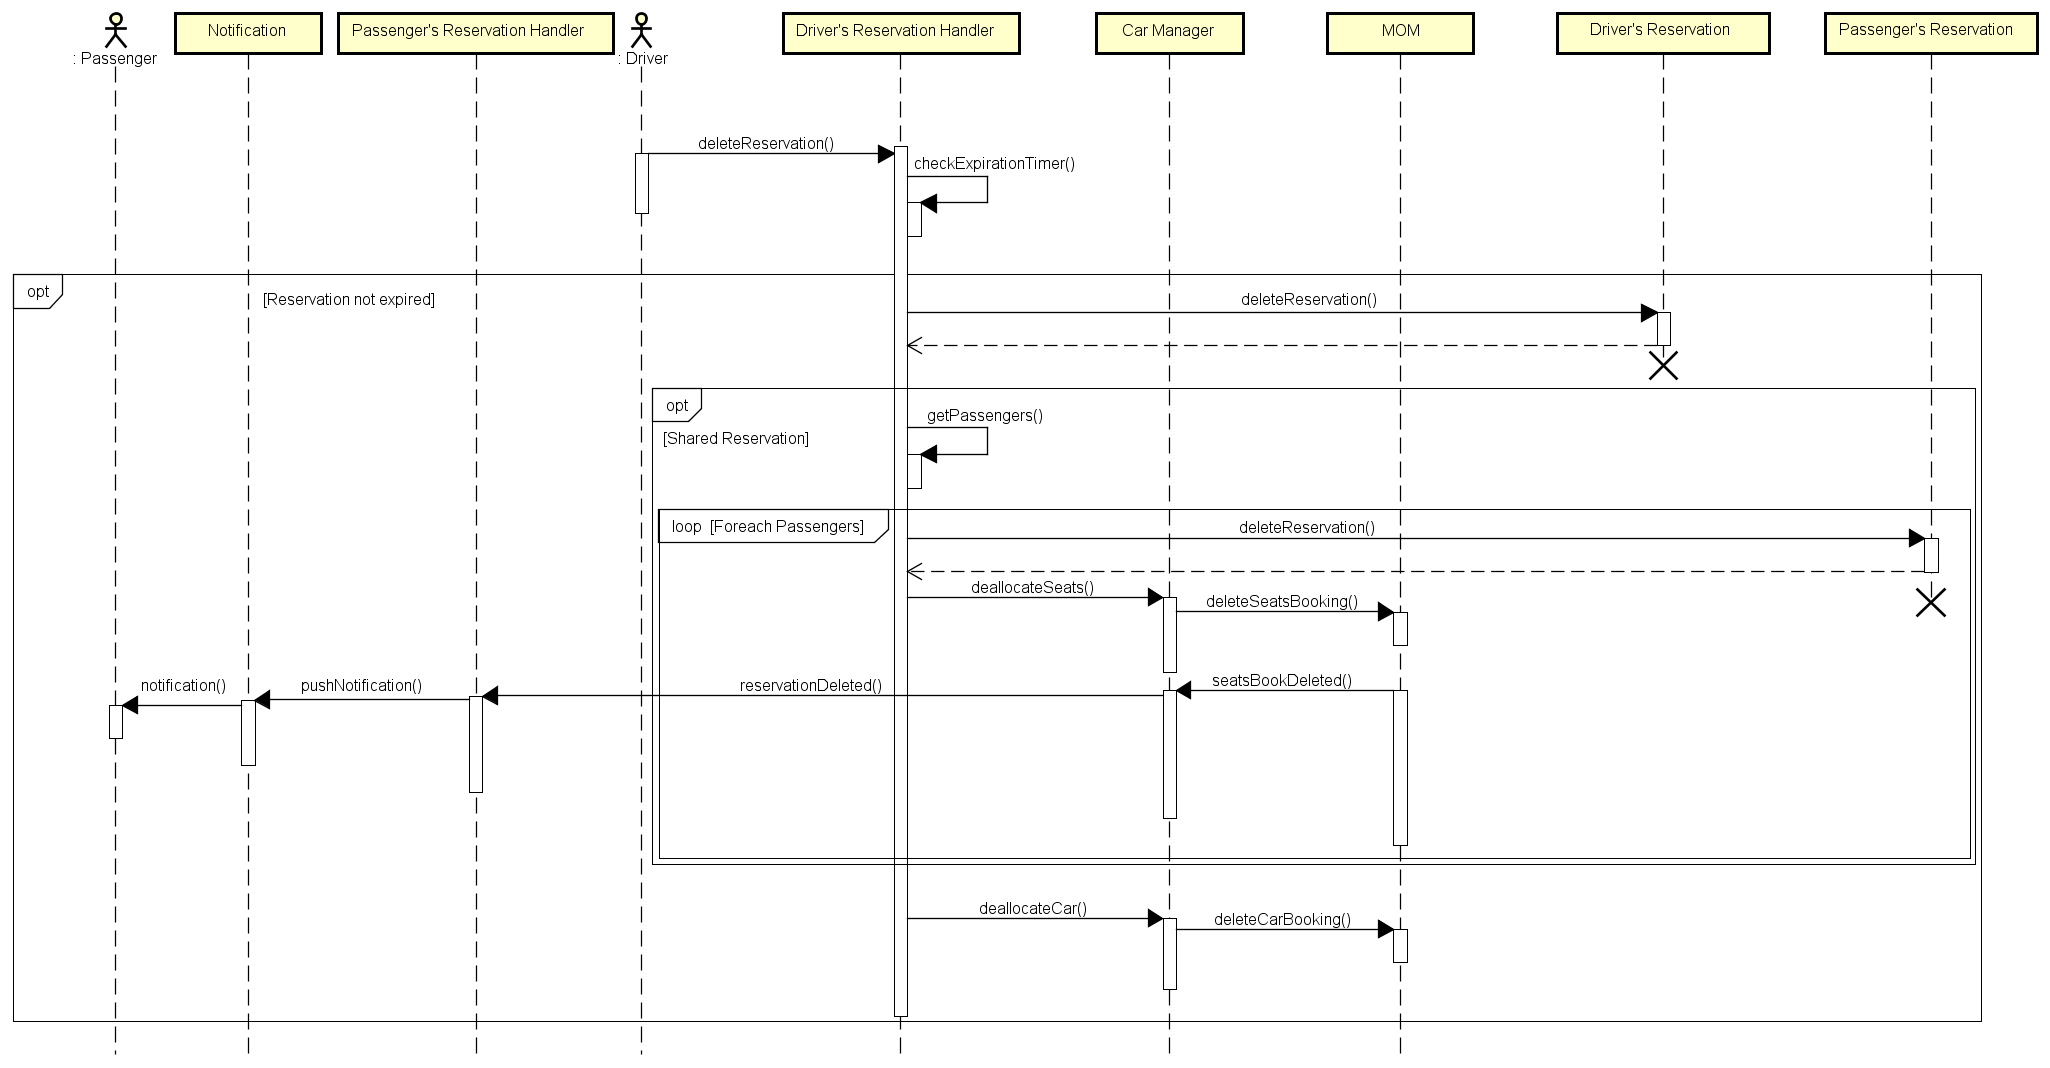
\includegraphics[keepaspectratio=true,scale=0.35]{../DD/img/sequence-diagram/delete-car-reservation}}
			\end{minipage}
			\begin{center}
				Image taken from the Design Document (paragraph 2.5.2.4)
			\end{center}
			\begin{center}
				\setlength{\tabcolsep}{24pt}
				\renewcommand{\arraystretch}{1.4}
				\begin{tabular}{ | l | p{8cm} |}\hline
					\textbf{Test procedure identifier} & TP6\\\hline
					\textbf{Purpose} & This test verifies the delete a car reservation procedure. The purpose of the procedure is to check the correct integration of all the involved components: Reservation Handler, Car Manager, MOM, Reservation and Notification. \\\hline
					\textbf{Procedure steps} & Execute in order IT3, IT4, IT12 and IT13 \\\hline
				\end{tabular}
			\end{center}
			\pagebreak
	\section{Tools and Test Equipment Required}
	To perform integration tests will be used the following software tools:
	\begin{itemize}
		\item Junit: for unit tests of the single components.
		\item Arquillian: for tests containers and their integration with JavaBeans.
		\item Mockito: for generate mock objects, stubs and drivers.
	\end{itemize}
	\section{Program Stubs and Test Data Required}
	In order to fulfill integration tests during the development, it is necessary to use stubs and drivers that will temporarily replace software components that do not yet exist.
		\subsection{Stubs}
			\begin{itemize}
				\item Payment Manager
				\item Notification
				\item Car Manager
				\item Payment service
				\item SMS service
				\item Email service
				\item Push notification service
				\item MOM
			\end{itemize}
		\subsection{Drivers}
			\begin{itemize}
				\item User (Passenger, Driver, Handyman Operator)
				\item Reservation Manager
				\item MOM
			\end{itemize}
		\subsection{Data required}
		To perform a correct integration testing it is necessary to implement a dummy DB that will contains a reduced set of instances and simulate MOM messages.
	\pagebreak
	\section{Effort Spent}
		\subsection{Hours of work} The time spent to redact this document:
		\begin{itemize}
			\item Bresich Matteo: 36 hours.
		\end{itemize}
		
		\begin{center}
			\begin{tabular}{ | l | l |}
				\hline
				Days & Hours of work\\ \hline
				02/01/17 & 6h\\\hline
				03/01/17 & 7h\\\hline
				04/01/17 & 7h\\\hline
				10/01/17 & 4h\\\hline
				11/01/17 & 4h\\\hline
				12/01/17 & 3h\\\hline
				13/01/17 & 2h\\\hline
				14/01/17 & 2h\\\hline
				15/01/17 & 1h\\\hline
				
			\end{tabular}
		\end{center}
	\section{References}
		\begin{itemize}
			\item TeXstudio v2.11.2 (http://www.texstudio.org/) to produce this document.
			\item Evolus Pencil v2.0.5 (http://pencil.evolus.vn/) to generate diagrams.
			\item Astah Professional 7.1.0 (http://astah.net/) to create Use Cases Diagrams, Sequence Diagrams, Class Diagrams and State Machine Diagrams.
		\end{itemize}
\end{document}